\section{The turbulence phase}
\label{sec:satTurb}
%
At a certain point the linear modes becomes large enough for non-linear effects to affect the dynamics of the system.
Through the non-linearities in the equation, mode-mode coupling occurs, leading to a cascading of enstrophy (global integrated vorticity) and energy.
The radial displacement of fluid parcels is much more restricted than the displacement along the field lines due to the magnetic field.
Consequently, the turbulence cascade have a more a 2 dimensional character than a 3 dimensional character.
In 2-D turbulence there is an inverse cascade of enstrophy as vortex stretching cannot occur.
In other words eddies tend to merge together to larger coherent structures.
This is something which is also seen in atmospheric flows, such as for example the great red spot on Jupiter.

FIXME: Back this up with references etc.

The main part of the energy is still cascading towards the smaller structures in 2-D turbulence.
At small enough scales the energy dissipates through diffusive processes.
The turbulence will reach a steady state once the input of energy through the source is balanced by the dissipation of energy.
On the transition from the linear phase to the turbulent phase a energy overshot is observed as seen in \cref{fig:energyTrace008}.
%
\begin{figure}[htb]
    \centering
    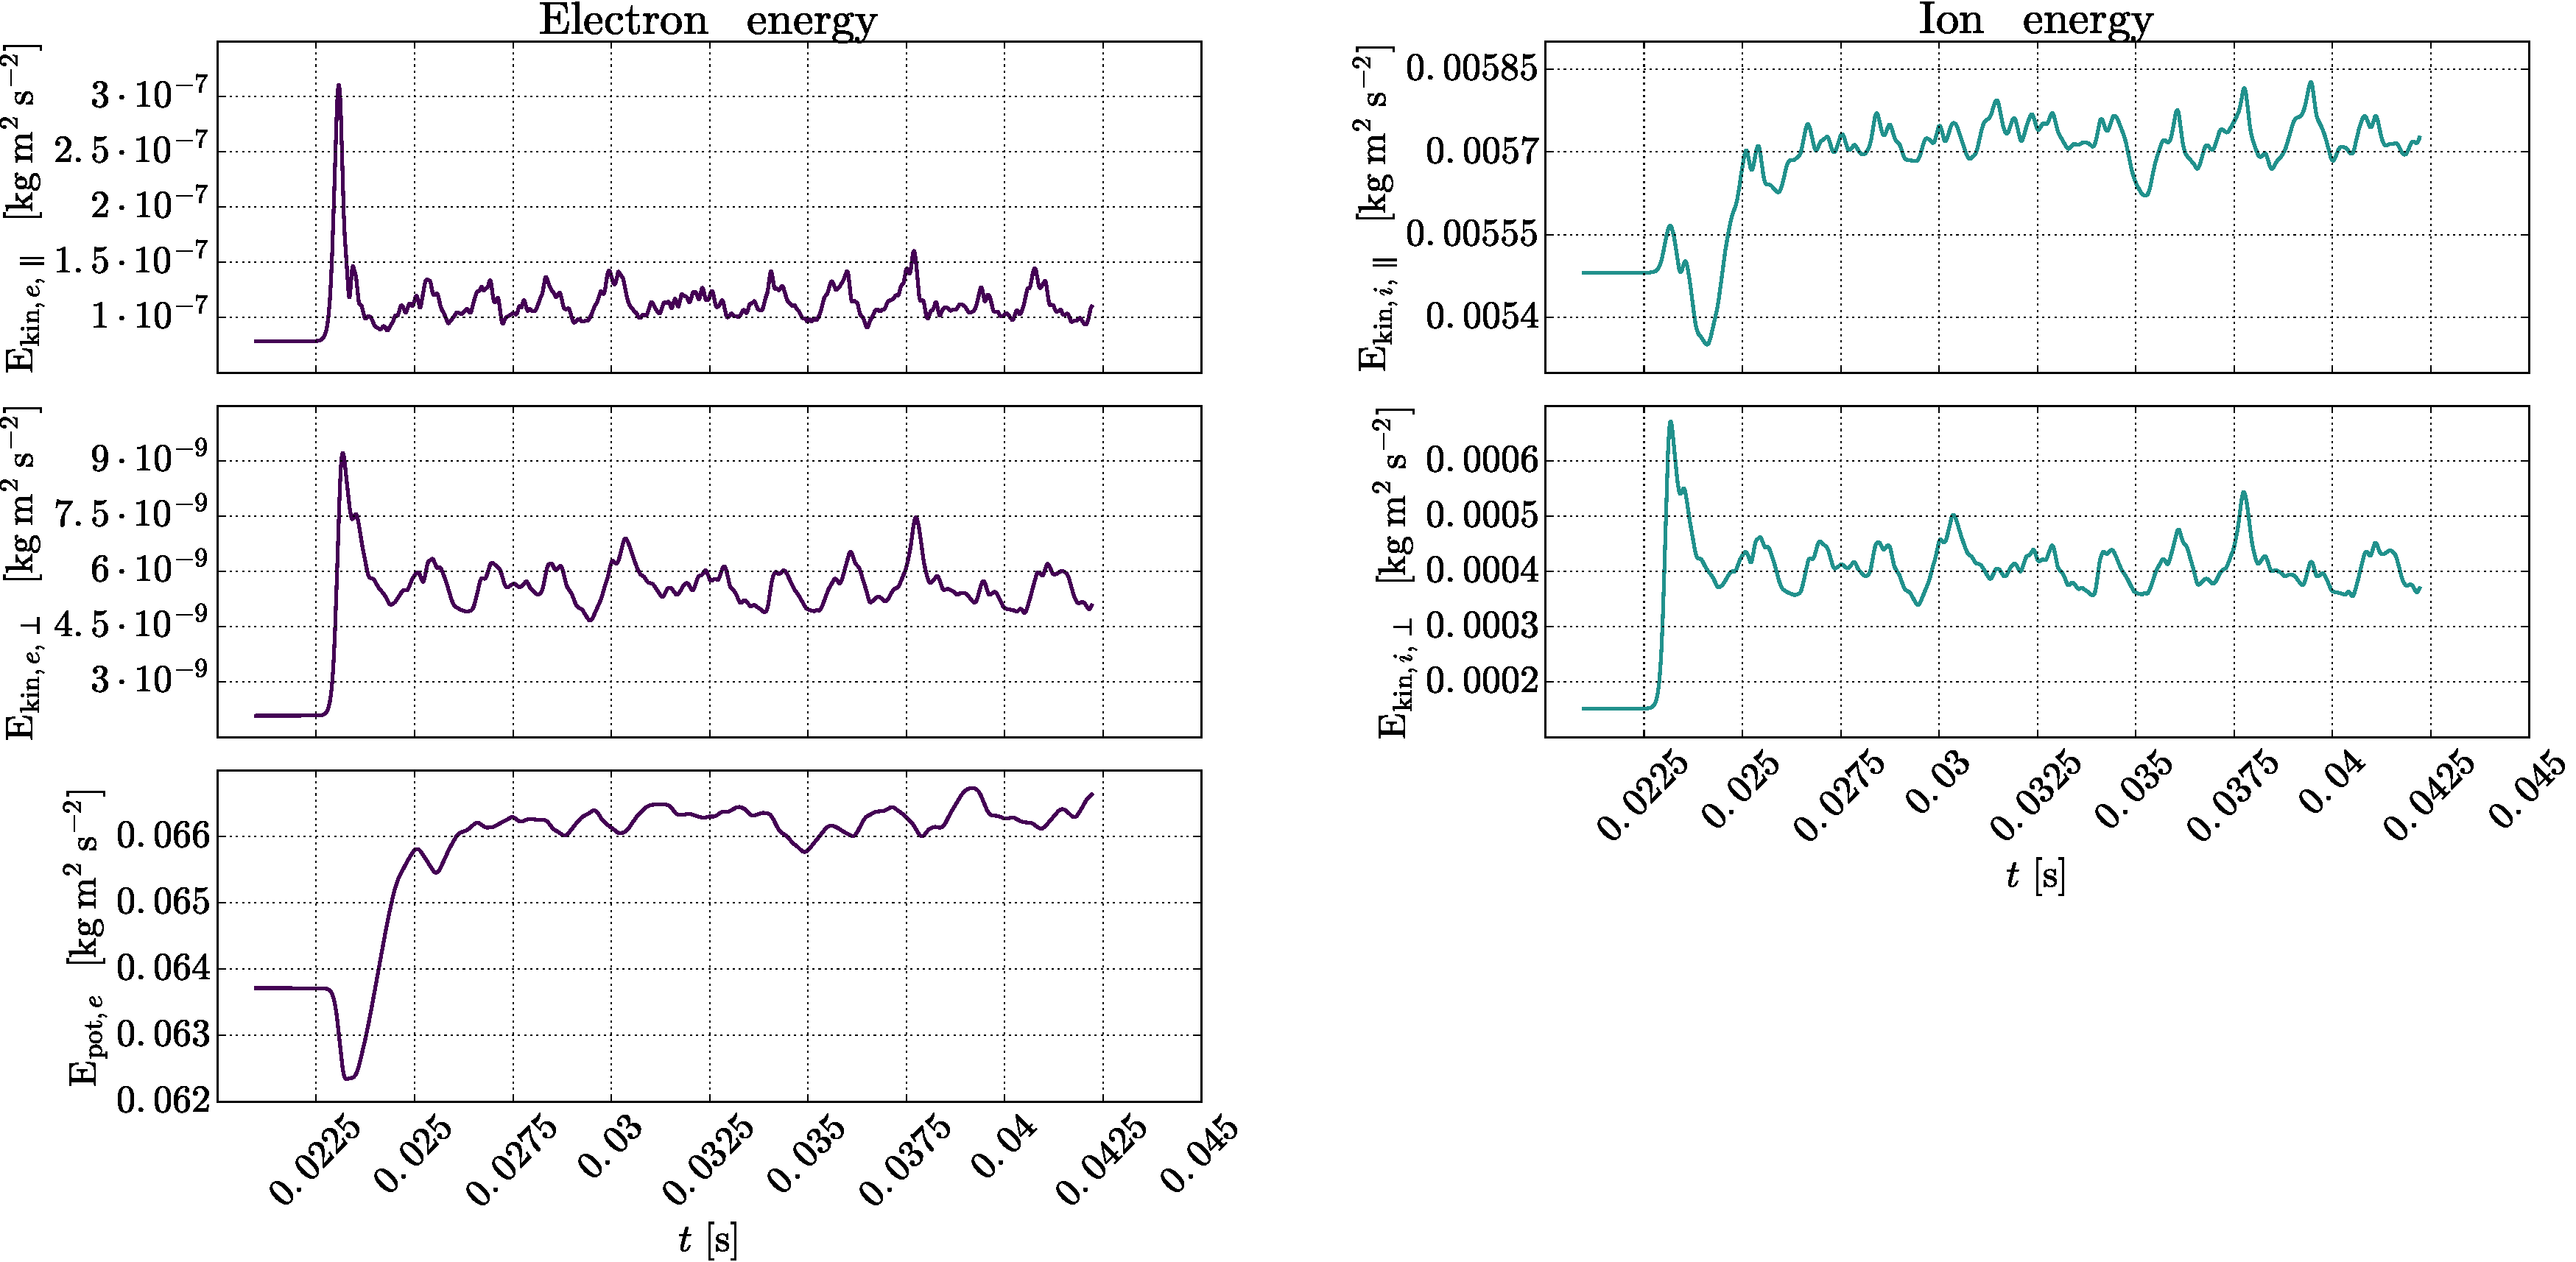
\includegraphics[width=1.0\textwidth]{fig/results/energyTrace/energyTraceB008}
    \caption{Time trace of the energy for $B=0.08$.}
    \label{fig:energyTrace008}
\end{figure}

As a consequence the eddies evolve at a faster phase at the transition as compared with the saturated turbulent state where eddies evolve at a slower rate.
In the saturated state the energy stays closer to the temporal mean, shown in \cref{fig:energyTrace008}.
It is also important to observe that the fluctuations can be big enough to push the plasma off center as observed in \cref{fig:turbEv}.
%
\begin{figure}[htbp]
    \centering
    \begin{subfigure}[h]{1.00\textwidth}
        \centering
        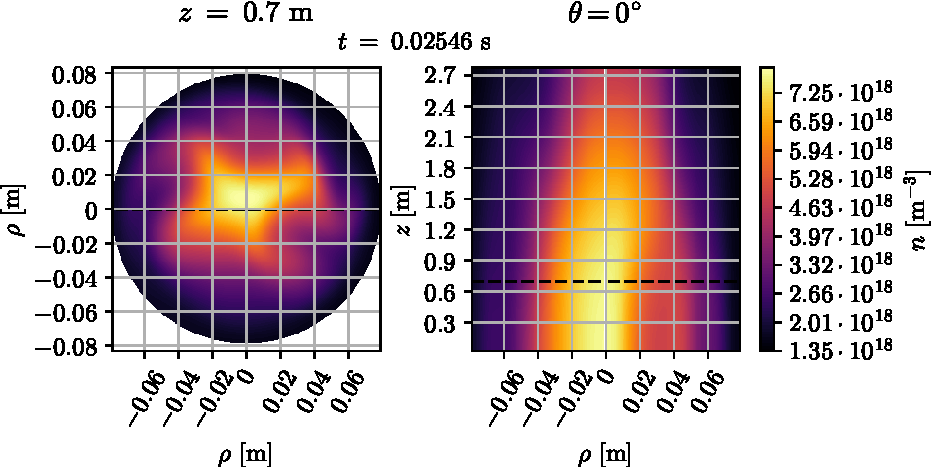
\includegraphics[width=1.0\textwidth]{fig/results/evolution/n-perpPar-2D-0}
    \end{subfigure}%
    \\
    \begin{subfigure}[h]{1.00\textwidth}
        \centering
        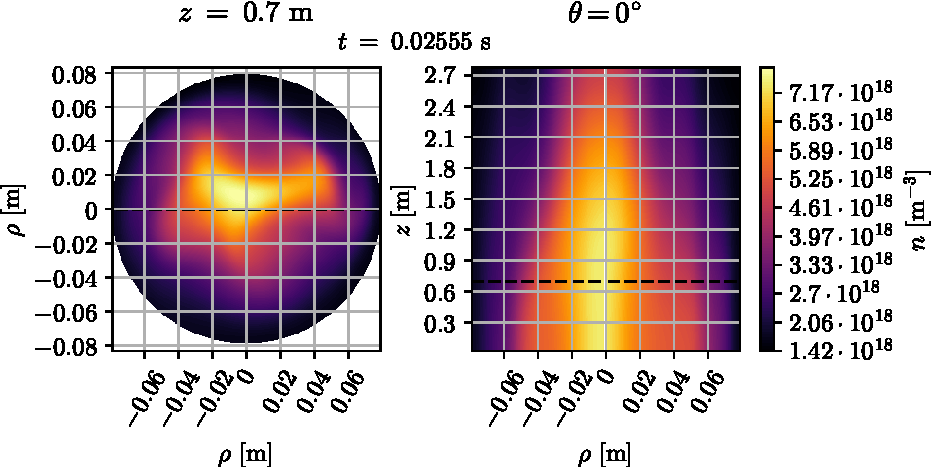
\includegraphics[width=1.0\textwidth]{fig/results/evolution/n-perpPar-2D-1}
    \end{subfigure}
    \\
    \begin{subfigure}[h]{1.00\textwidth}
        \centering
        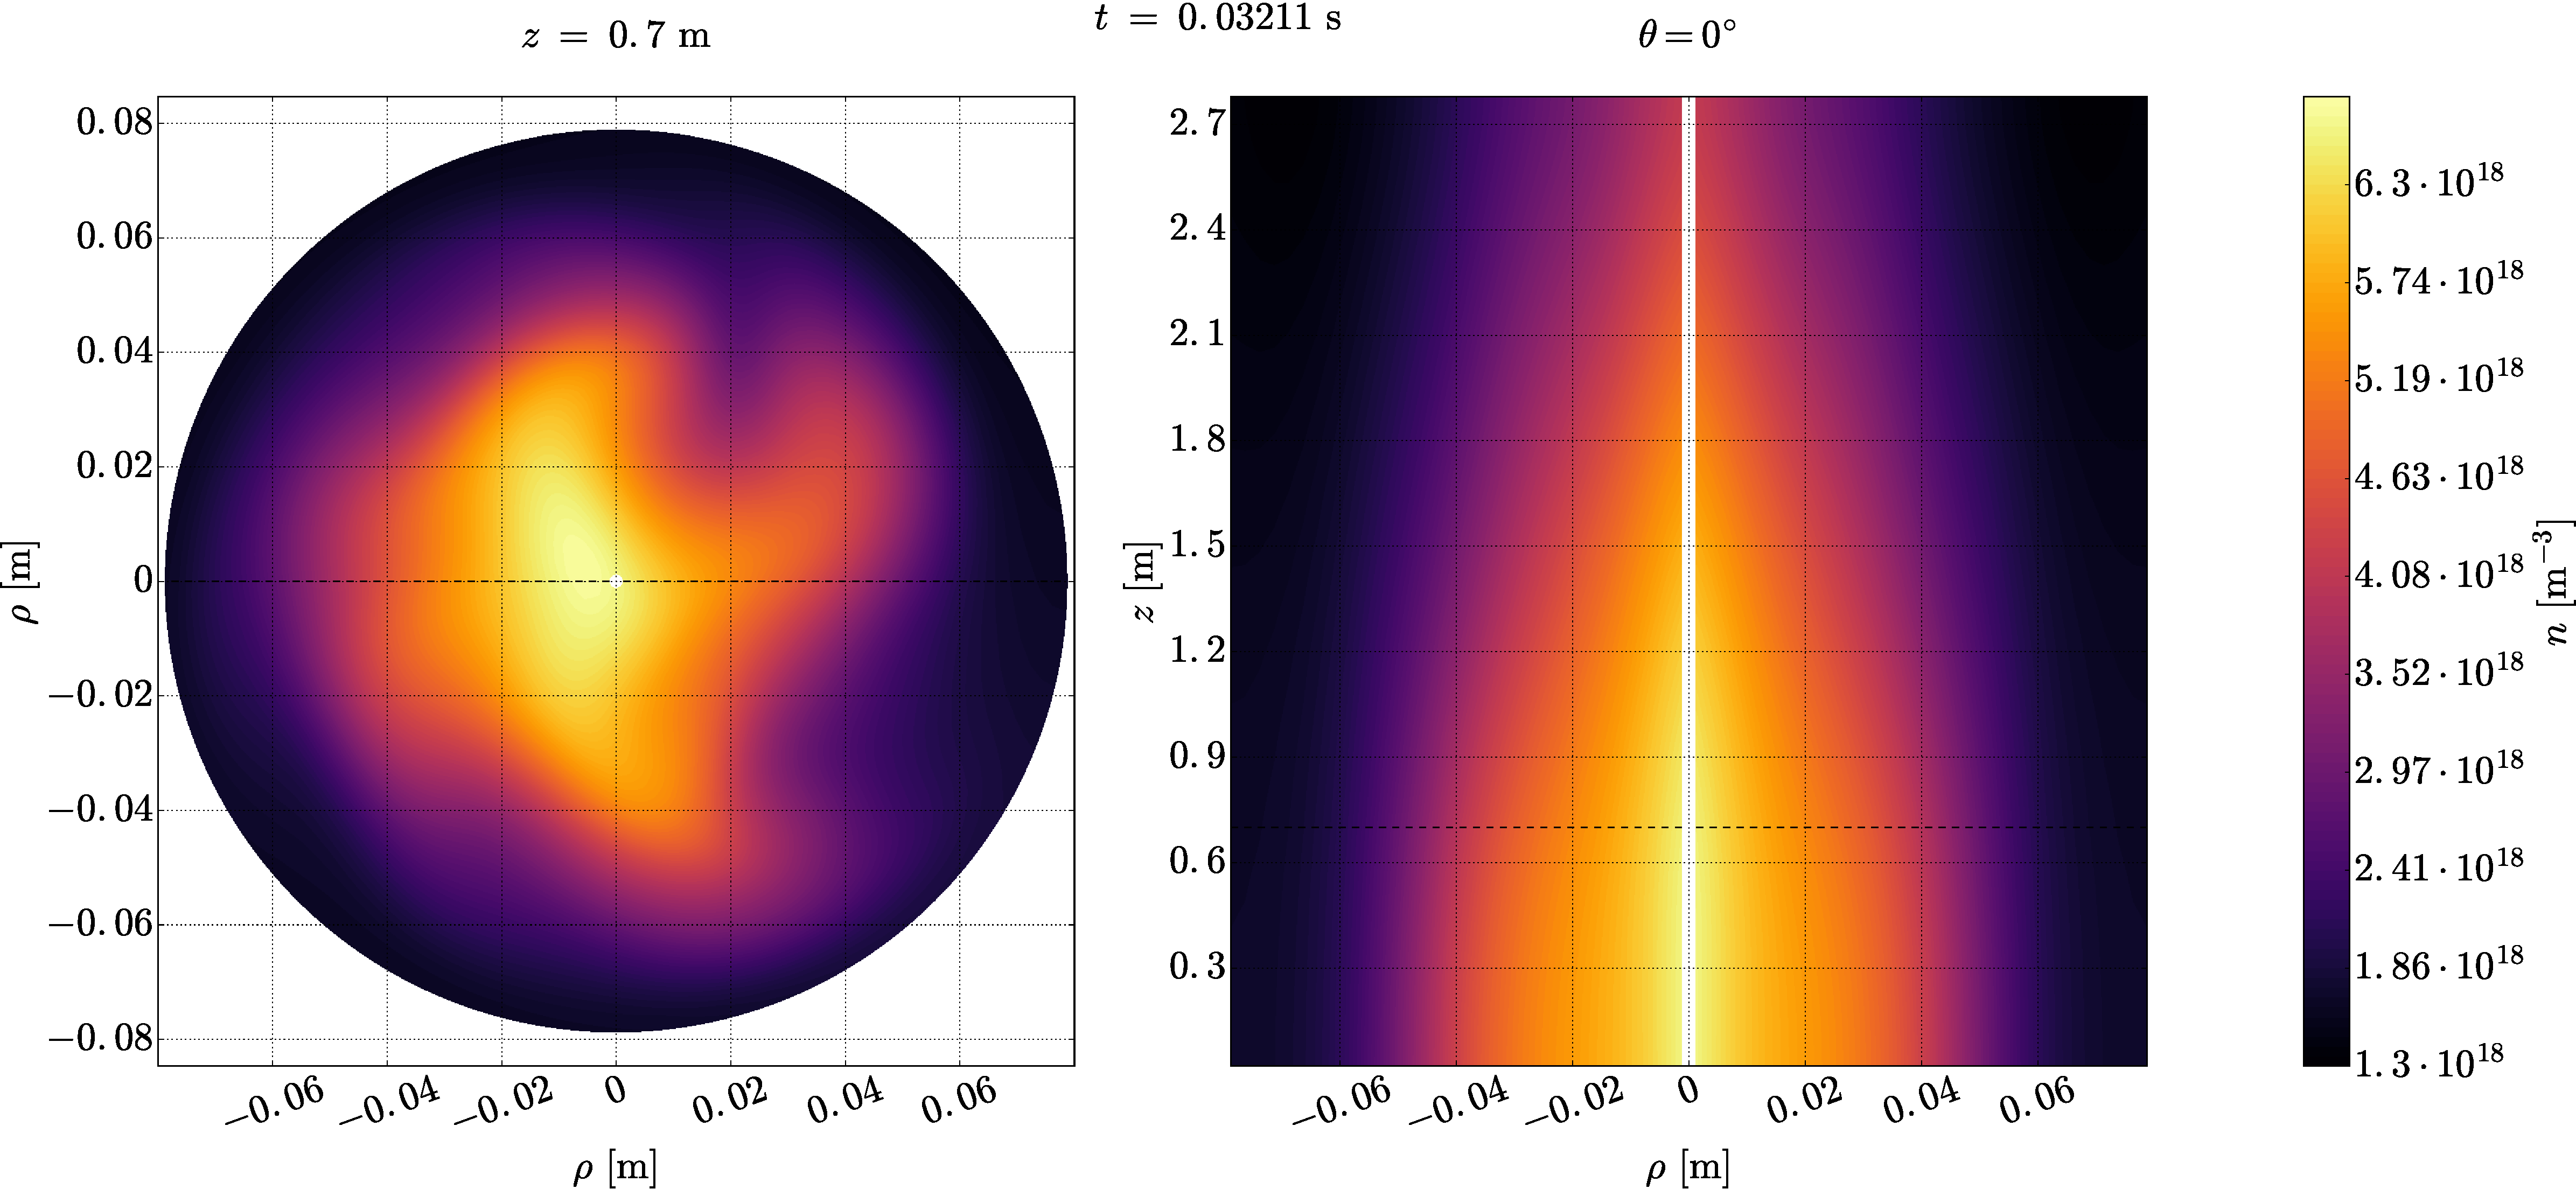
\includegraphics[width=1.0\textwidth]{fig/results/evolution/n-perpPar-2D-2}
    \end{subfigure}
    \caption{Evolution of the plasma in the saturated turbulence phase.
        Here shown for $B=0.08\T$}
    \label{fig:turbEv}
\end{figure}
%
In the saturated turbulence state, the fluctuations are no longer in an ordered pattern as they were in the linear phase.
\Cref{fig:2DFluct} shows this.
%
\begin{figure}[htb]
    \centering
    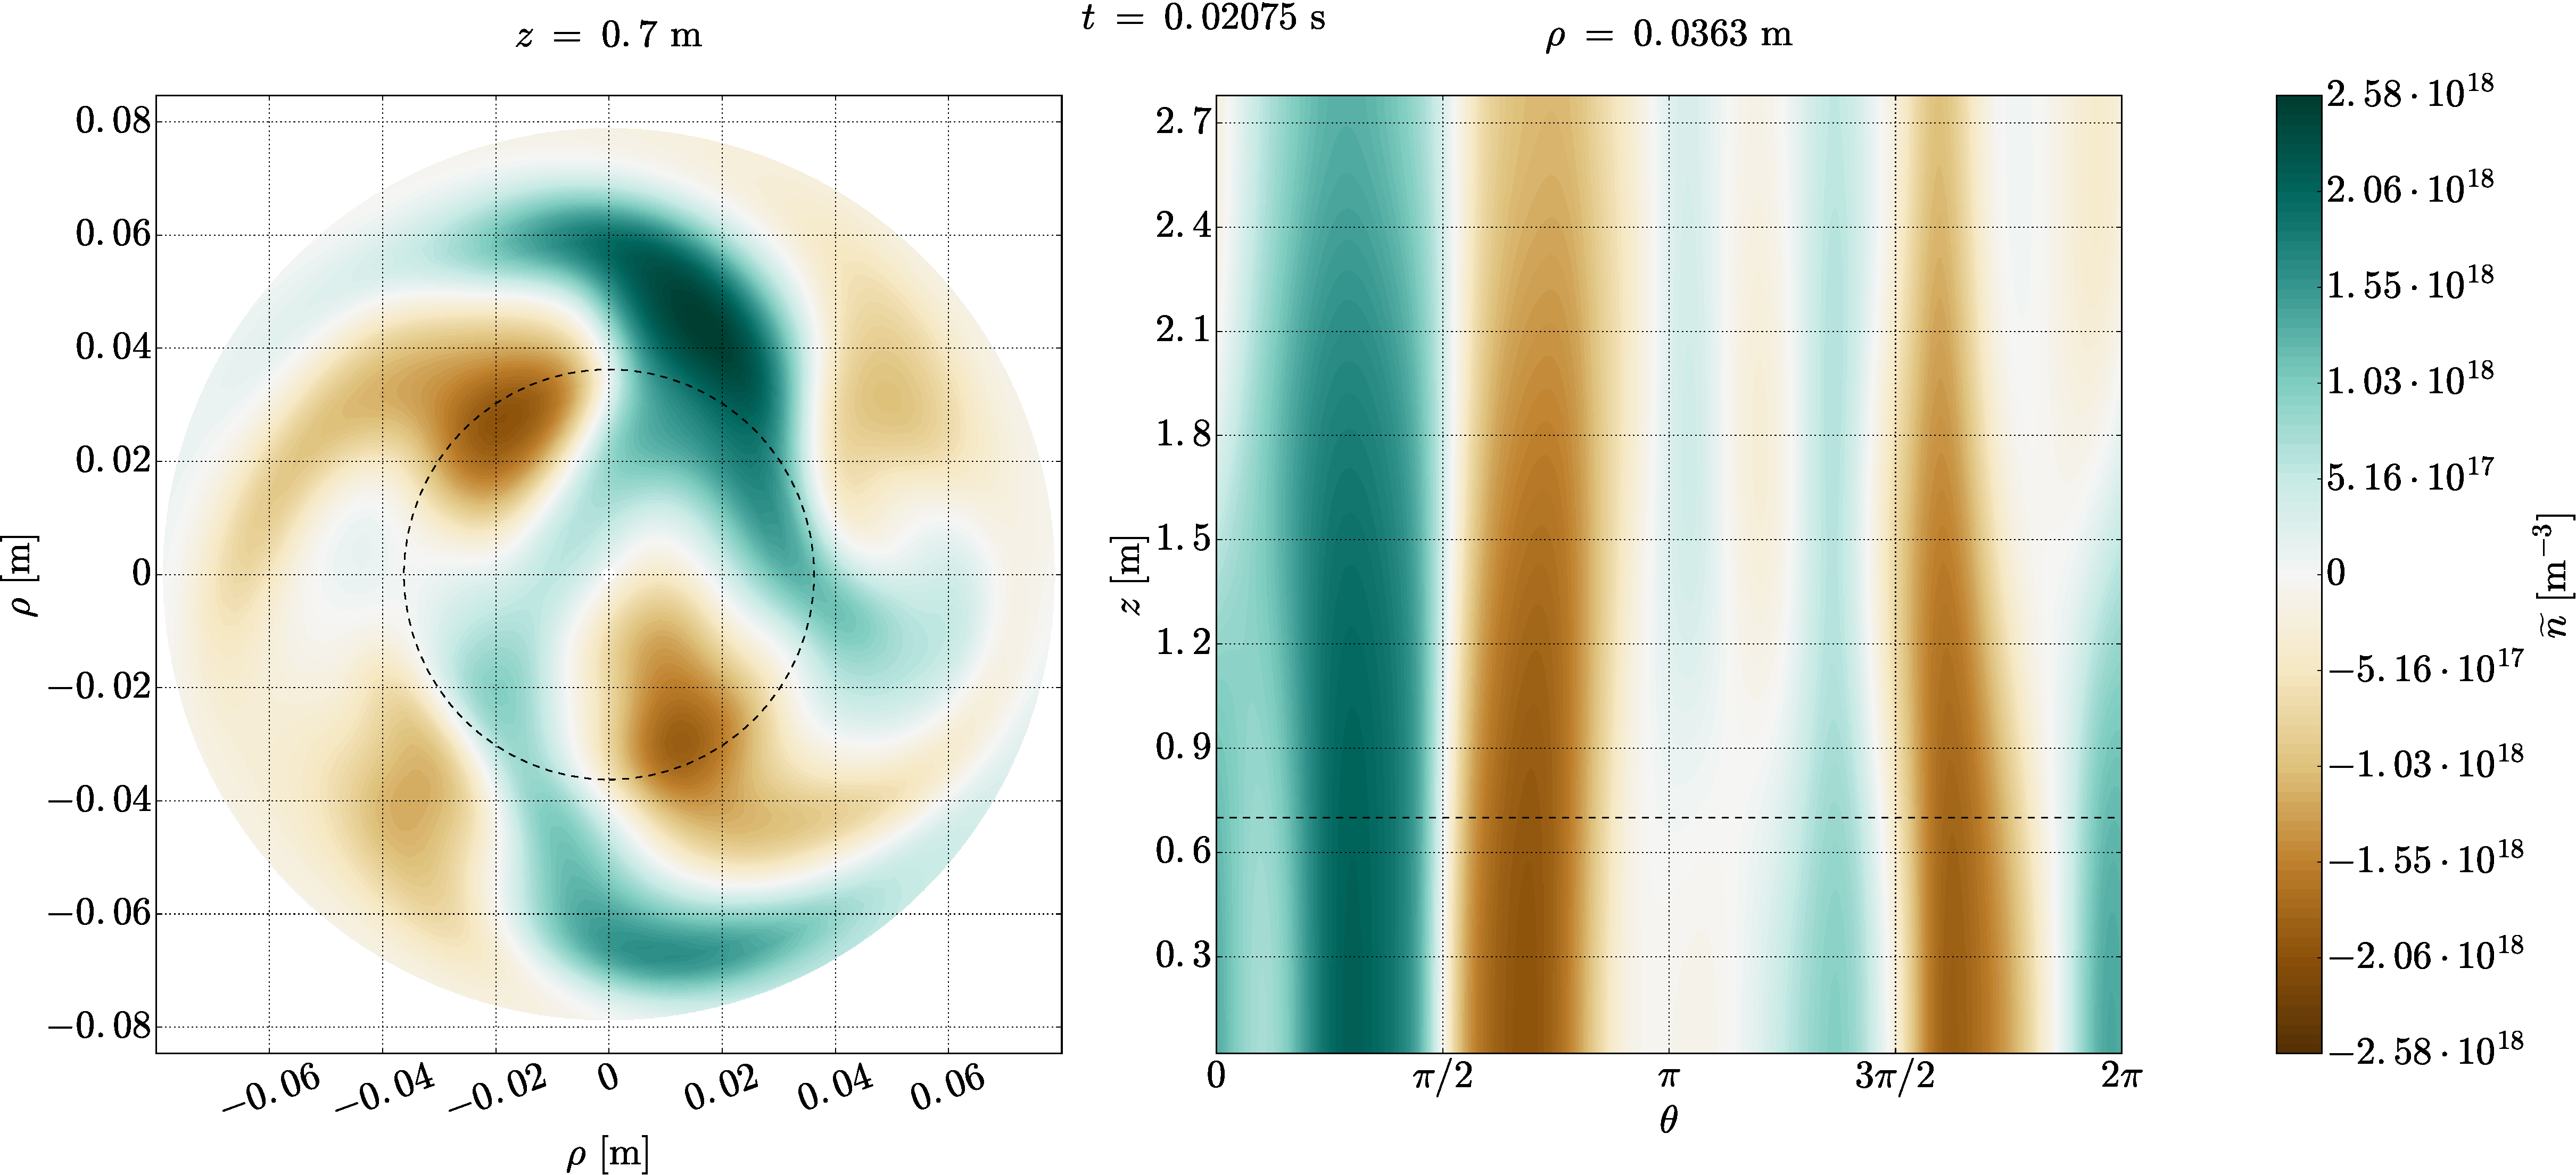
\includegraphics[width=1.0\textwidth]{fig/results/2DTurbulence/fluct}
    \caption{Fluctuations in the turbulent state for $B=0.1\T$}
    \label{fig:2DFluct}
\end{figure}
%
\subsection{Fluxes}
FIXME: Move figures and describe
%
\begin{figure}[htb]
    \centering
    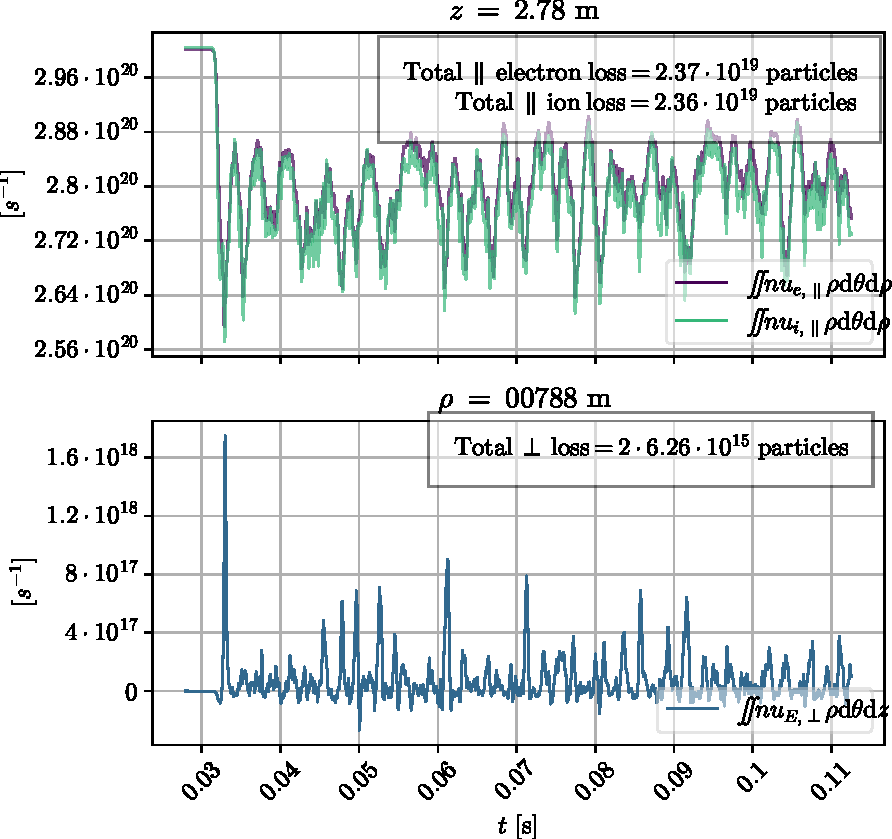
\includegraphics{fig/results/totalFlux/flux0008}
    \caption{Integrated flux for $B=0.08\T$}
    \label{fig:flux0008}
\end{figure}
%
\begin{figure}[htb]
    \centering
    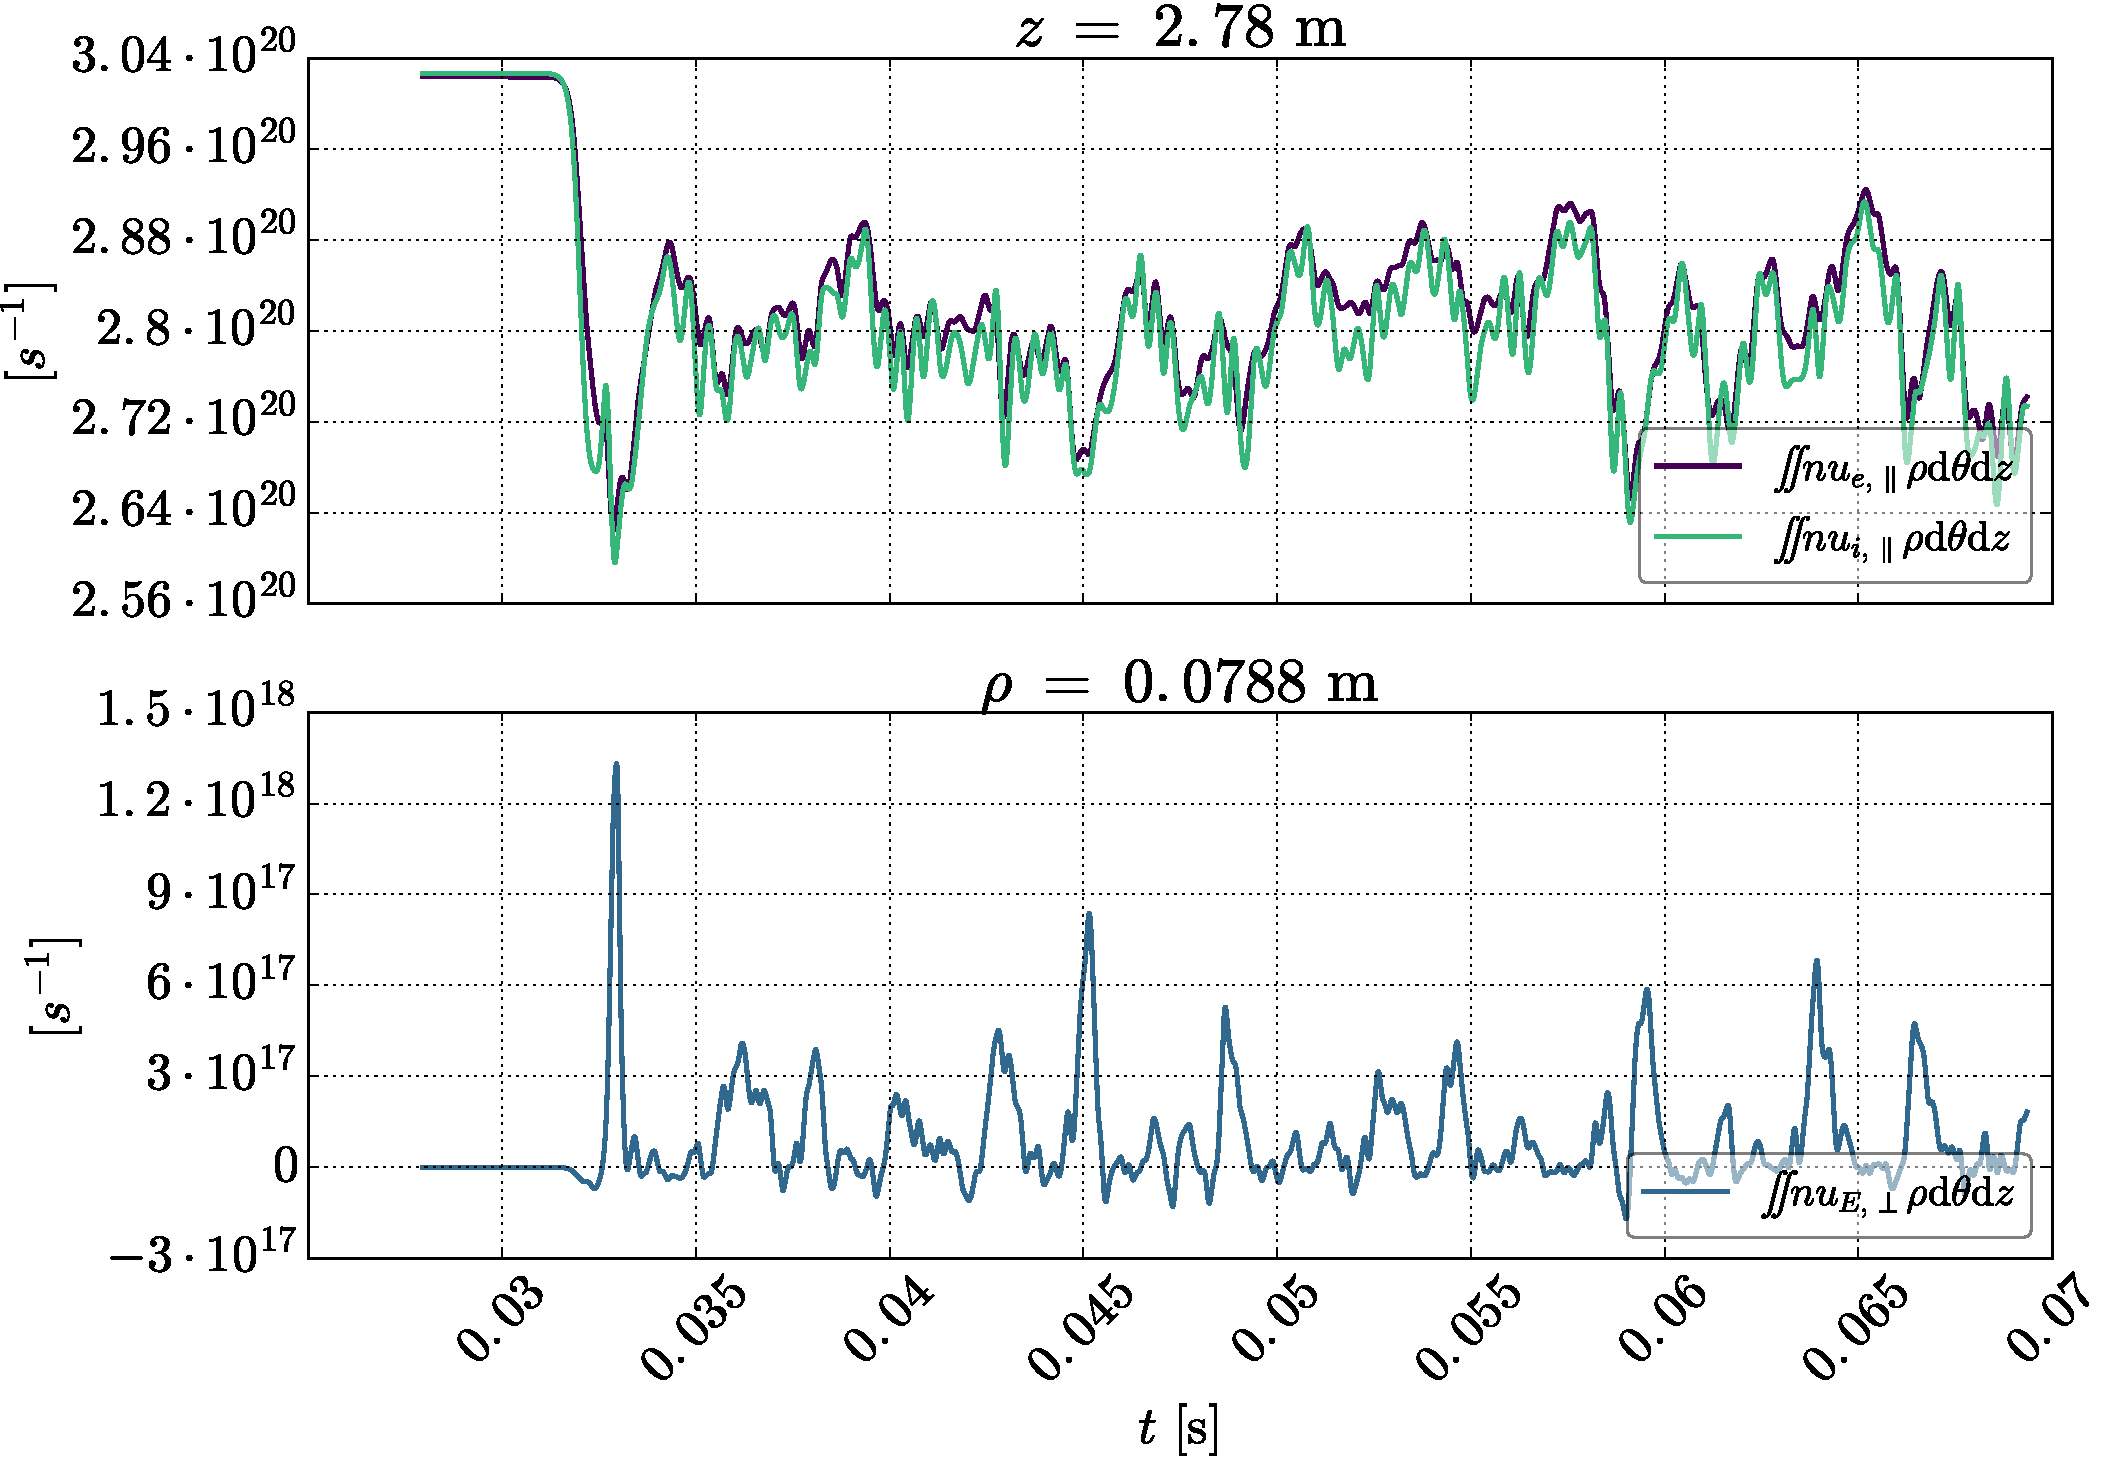
\includegraphics{fig/results/totalFlux/flux0006}
    \caption{Integrated flux for $B=0.06\T$}
    \label{fig:flux0006}
\end{figure}
